In order to test our data, we have decided to make use of a random data generator.
Our reasoning is that while we could use real data from open source repositories, a dedicated generator will allow us
to build data in the shape that we choose to test, this is beneficial for:

- large dataset testing: as we can generate datasets of arbitrary size

- data trend testing: as we can build our own custom trends, without having to analyse and understand real life trends

- data inconsistency: as we can introduce purpose built inconsistencies, this will help if we build tools that operate on specific error margins

Concerns regarding random data accurately modelling real life data will be addressed at the end of this section.

\subsection{Implementation (iteration 1)}\label{subsec:implementation-(iteration-1)}
For our first draft of the implementation, we have kept the feature list simple.

\begin{figure}[h]
    \centering
    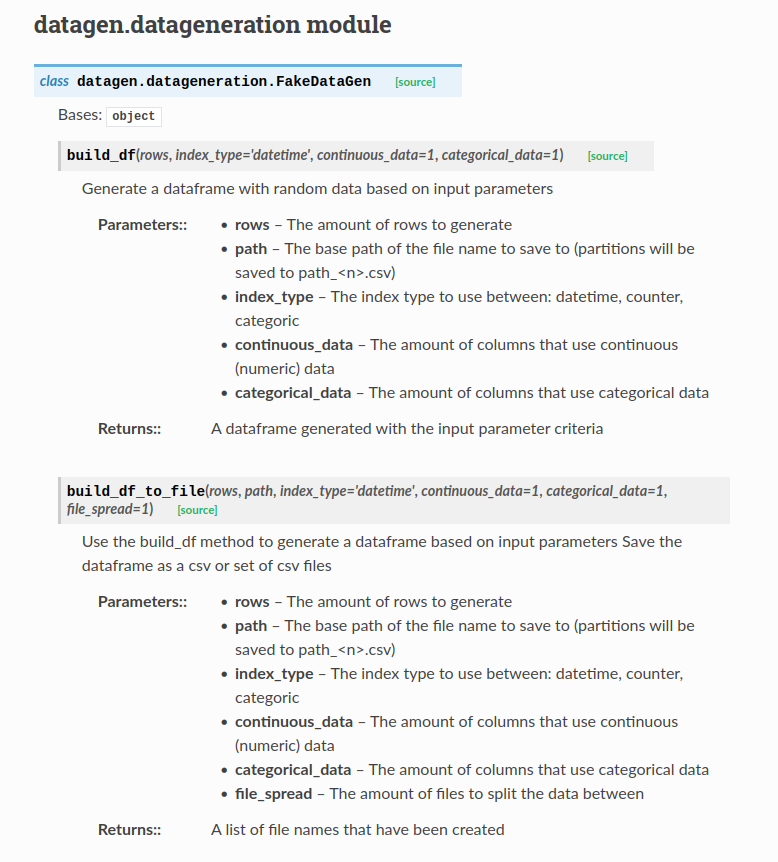
\includegraphics[width=12cm]{figures/data_generation/datagen_doc_v1}
    \caption{Documentation overview for the data generation implementation}
    \label{fig:datagen_doc_1}
\end{figure}

As summarised in the documentation in\ref{fig:datagen_doc_1} we expose functionality to create a table that has a
parameterised amount of rows and columns, with columns either being numeric or categorical.
Column names are generated using random words, and the index column can be defined in three different formats:

- counter: The simplest one, the index is just an index that increments by 1

- datetime: Starting at 2016, each row in the index is a datetime that increments by 1 day

- categorical: Each index is a generated UUID

For numeric data, we chose to start off by modeling a sin wave with slight variance, which would easy to calculate, and
would resemble simple repeating trends

\begin{figure}[h]
    \centering
    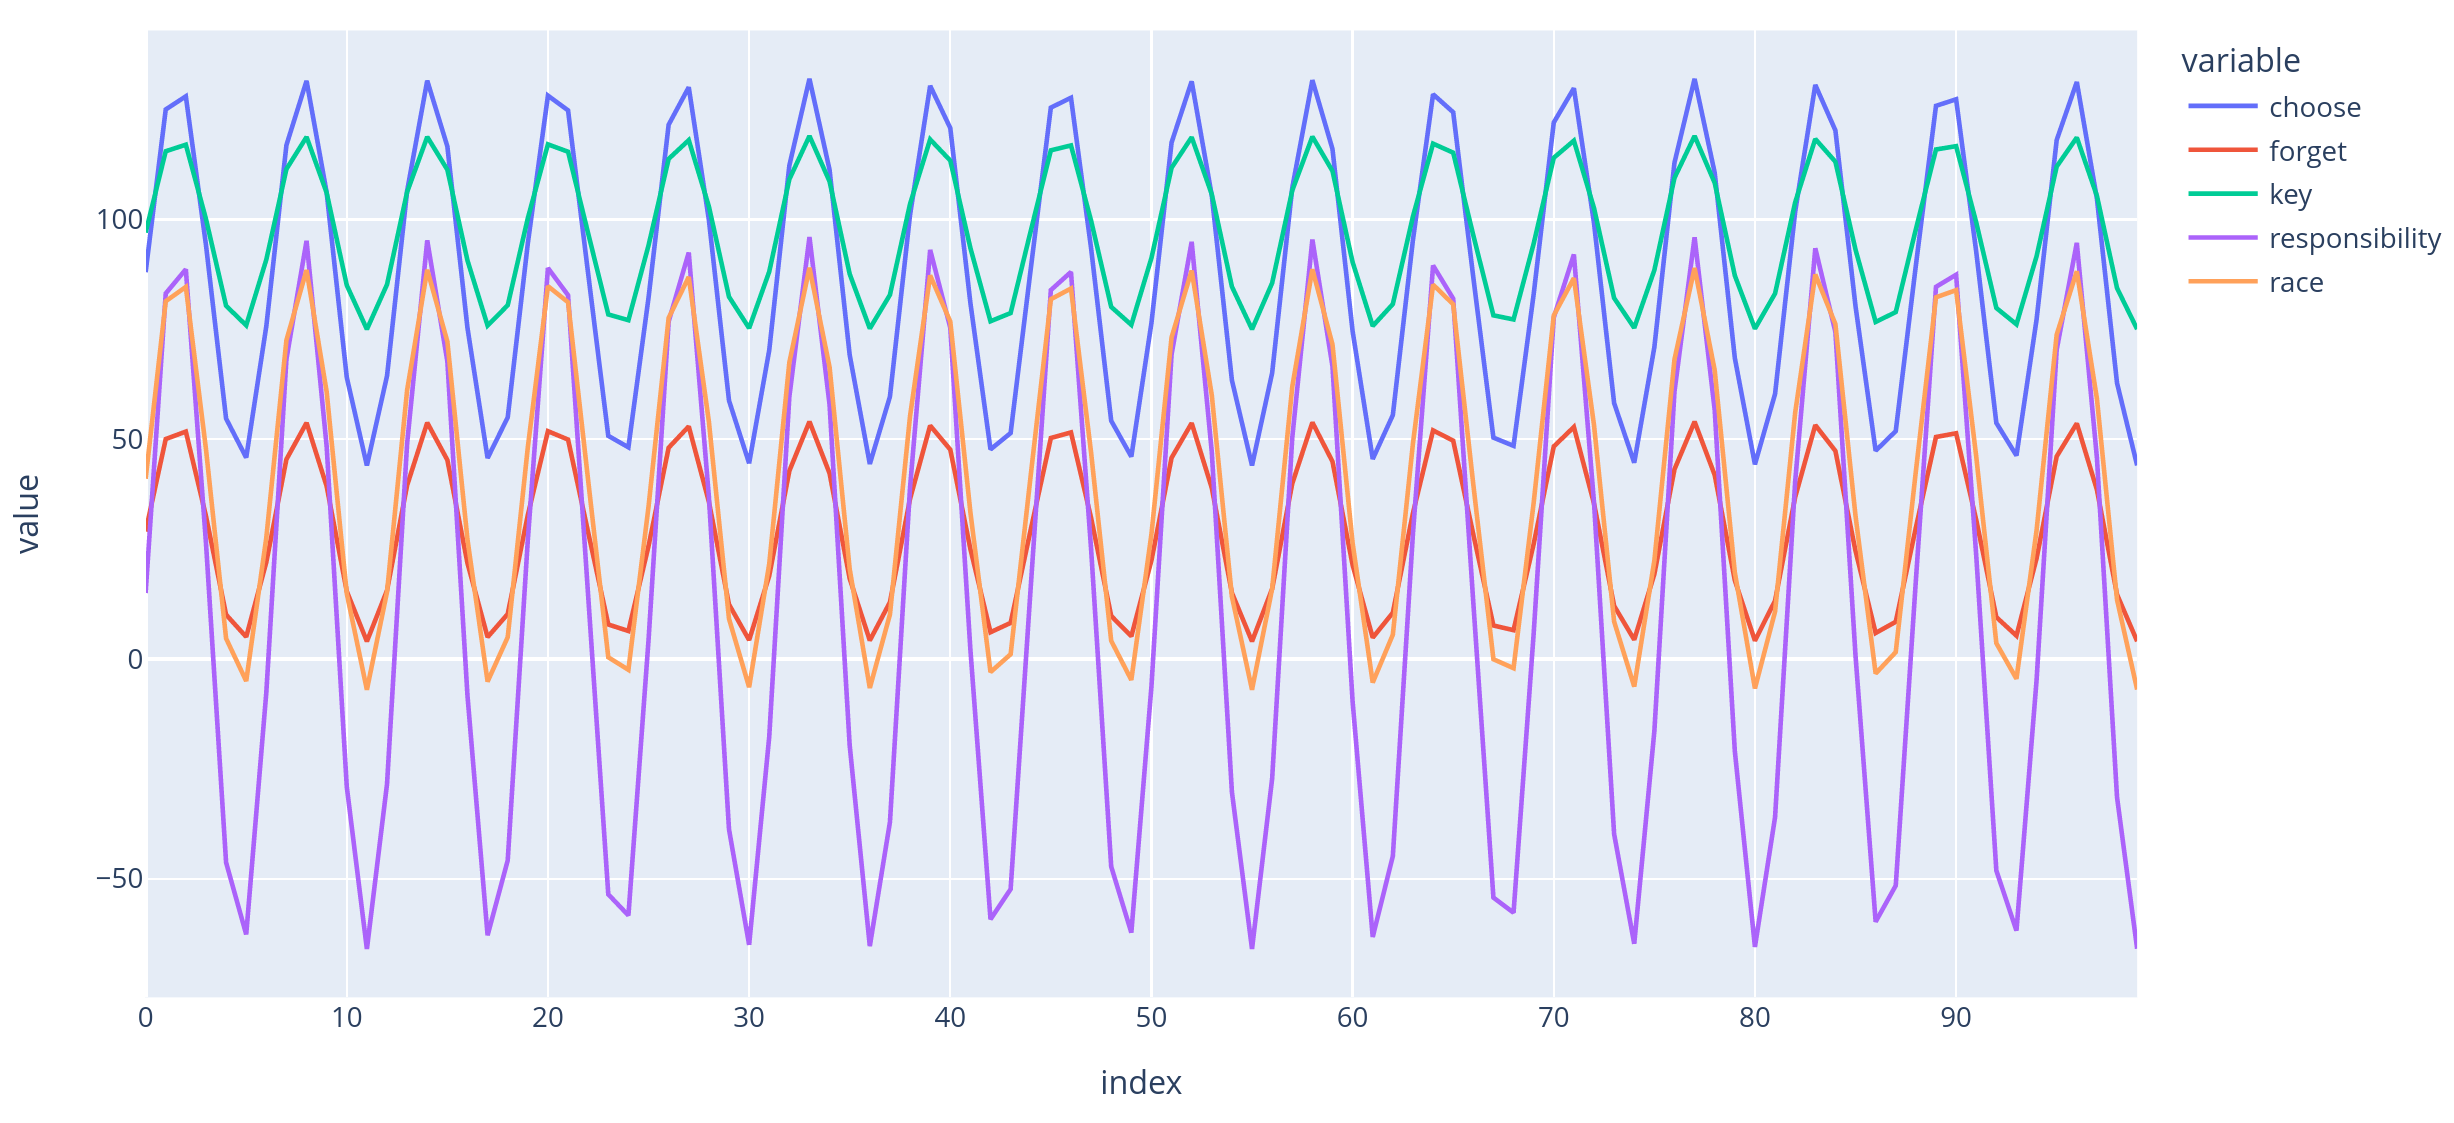
\includegraphics[width=12cm]{figures/data_generation/fake_data_gen_continuous_1}
    \caption{Visualisation of the data generation with 100 rows and 5 continuous columns, note that sin waves are all in phase}
    \label{fig:datagen_fig_1}
\end{figure}

For categorical data, we used the faker(TODO: REF HERE?) library to generate random words for each cell.

While our first draft does not do a good job of modelling real world data, a lot of our discovery client features do not
require any knowledge of the data, so this is an acceptably complete product until such features need to be tested.

In terms of performance, we try to use as little task switching as possible - this means that functions such as creating
a UUID, or getting a faker name, will both slow down processing time a lot.
In future iterations it may be beneficial to put more effort into preventing these calls from happening with each row,
and introducing a multithreaded approach to building larger dataframes.
There is also a slight issue that creating a large spread of files will still start by building a single dataframe, which
may cause memory issues for larger sets of smaller data (this can be avoided by building each file individually).

\subsection{Implementation (iteration 2)}\label{subsec:implementation-(iteration-2)}

In this iteration we approach the issues mentioned in the last section.

We start by abstracting the concept of a column into its own class, which allows us to build an arbitrary dataframe
based on the specified columns.

Our next change is to transform columns into infinite data generators, when generating large datasets, we can specify
a chunk size, and write to files without holding data in memory.

Now that columns are abstracted, we can approach each type of data column we would like to emulate individually:

\subsubsection{Linear}

The most simple type of numerical data, returns a series that can be plotted as y=x


\subsubsection{SinWave}

Similar to the sin wave implemented in the first iteration, we count upwards and apply the sin function to the number.
In the future it may be worth resetting the counter occasionally, which will prevent the counter from becoming too large
and using more memory.

We provide additional options that allow more varied data sets:

- \textbf{variance}: The variance of plot points on the y-axis

- \textbf{phase variance}: The variance of plot points on the x-axis

- \textbf{noise}: Generate a random number to modify each plot point


\subsubsection{Random Word}

Generate a random word using the faker library
